% -*- TeX:PL -*-
% $Id: $
\documentclass[17pt]{beamer}
\usepackage[T1]{polski}
\usepackage[utf8]{inputenc}
\usepackage{lipsum}
\usepackage{multimedia}

\author{}
\title{Opracowanie inteligentnego systemu sterowania ruchem drogowym}
 \subtitle{}
 \date{}
 \institute{autor: inż. Przemysław Rokosz\\\vspace{\baselineskip}promotor: dr inż. Grzegorz Filcek}
 \subject{Opracowanie inteligentnego systemu sterowania ruchem drogowym}
 \keywords{Inteligentny System Sterowania Ruchem Drogowym}
 \titlegraphic{}

\DeclareGraphicsExtensions{.pdf,.png,.jpg}

\setbeamersize{text margin left=0mm,text margin right=2.5mm}
\usetheme[]{pwr}

\setbeamertemplate{footline}
{
\leavevmode
\hbox{
\begin{beamercolorbox}[wd=.88\paperwidth,ht=2.5ex,dp=1.125ex,right]{title in head/foot}
\end{beamercolorbox}
\begin{beamercolorbox}[wd=.1\paperwidth,ht=2.5ex,dp=1.125ex,center]{title in head/foot}
\usebeamerfont{author in head/foot} \insertframenumber/\inserttotalframenumber
\end{beamercolorbox}
}
\vskip0pt%
}

\setbeamertemplate{navigation symbols}{}

\hypersetup{
 urlcolor=blue
}

\begin{document}
\begin{frame}[plain,t]
 \maketitle
\end{frame}

\begin{frame}[shrink=5]
 \frametitle{\vspace{22px}Plan prezentacji}
 \begin{itemize}
  \item{Sterowanie ruchem drogowym}
  \item{Cel pracy}
  \item{Opis opracowanego systemu}
  \item{Wyniki badań}
  \item{Wnioski}
 \end{itemize}
\end{frame}

\begin{frame}[shrink=5]
 \frametitle{\vspace{22px}Sterowanie ruchem drogowym}
 Podstawowe zadania sterowania ruchem
 \begin{itemize}
  \item{Maksymalizacja wykorzystania dróg}
  \item{Zapobieganie tworzenia się korków}
  \item{Poprawa bezpieczeństwa ruchu}
 \end{itemize}
 Wyzwania sterowania ruchem
 \begin{itemize}
  \item{Niedeterministyczny charakter ruchu}
  \item{Nie zawsze możemy przewidzieć trasę pojazdu}
 \end{itemize}
\end{frame}

\begin{frame}[shrink=5]
 \frametitle{\vspace{22px}Cel pracy}
 Próba opracowania inteligentnego, adaptacyjnego, systemu sterowania ruchem drogowym na obszarze wzorowanym na okolicach placu Grunwaldzkiego we Wrocławiu.\\
 Porównanie opracowanego algorytmu sterowania ruchem z prostym algorytmem sterowania i brakiem sterowania.\\
\end{frame}

\begin{frame}[shrink=5]
 \frametitle{\vspace{22px}Cel pracy}
Stworzenie systemu który będzie dynamicznie reagował na zmienną charakterystykę ruchu drogowego oraz będzie stosował się do, wymaganych przez prawo, ograniczeń.
\end{frame}

\begin{frame}[shrink=5]
 \frametitle{\vspace{22px}Model opracowanego systemu}
 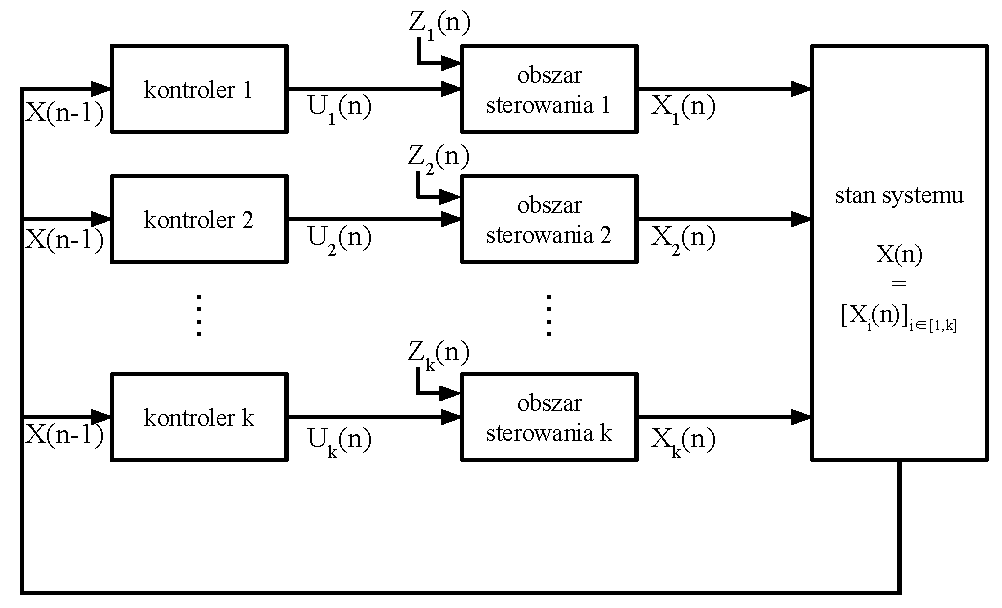
\includegraphics[width=1.0\textwidth]{model.pdf}
  \tiny{
  \begin{description}
   \item[U] -- wyznaczone przez kontrolery sterowania sygnalizatorów\\
   \item[X] -- stan systemu - wartości czujników i stany sygnalizatorów\\
   \item[Z] -- przepływ pojazdów wjeżdżających do danego obszaru sterowania\\
  \end{description}
   }
\end{frame}

\begin{frame}%[shrink=5]
  \scriptsize {
  \frametitle{\vspace{22px}Algorytm}
  \begin{enumerate}
    \item Wyznaczenie wszystkich, możliwych decyzji w postaci zbiorów bezkolizyjnych ustawień sygnalizatorów
    \item Wyliczenie wag sygnalizatorów
    \item Wyliczenie wartości funkcji oceny jako sumy wag sygnalizatorów zezwalających na ruch w ramach tej decyzji, dla wyznaczonych wcześniej możliwych decyzji
    \item Wyznaczenie optymalnej, o najwyższej wartości funkcji oceny, decyzji
    \item Wyznaczenie sekwencji sygnałów doprowadzających ustawienia sygnalizatorów do ustwień optymalnej decyzji
  \end{enumerate}
  }
\end{frame}

\begin{frame}[shrink=5]
  \frametitle{\vspace{22px}Algorytm - waga sygnalizatora}
  $$w = p \cdot \frac{f}{m} + q \cdot \frac{y_{1}}{m} + r \cdot \frac{y_{2}}{k_{i}}$$\\
  \tiny{
  \begin{math} w_{i} \end{math} -- waga sygnalizatora\\
  \begin{math} f \end{math} -- przewidywany przepływ pojazdów z sąsiedniego obszarun\\
  \begin{math} y_{1} \end{math} -- aktualny przepływ pojazdów przed sygnalizatorem\\
  \begin{math} y_{2} \end{math} -- aktualna wielkość kolejki przed sygnalizatorem\\
  \begin{math} m \end{math} -- maksymalny możliwy do zmierzenia przepływ pojazdów\\
  \begin{math} k \end{math} -- maksymalna wielkość kolejki przed sygnalizatorem\\
  \begin{math} p \end{math} -- wpływ przewidywanego przepływu pojazdów na sterowanie\\
  \begin{math} q \end{math} -- wpływ aktualnego przepływu pojazdów na sterowanie\\
  \begin{math} r \end{math} -- wpływ aktualnej kolejki na sterowanie\\
  }
\end{frame}

\begin{frame}[shrink=5]
  \frametitle{\vspace{22px}Badany obszar}
  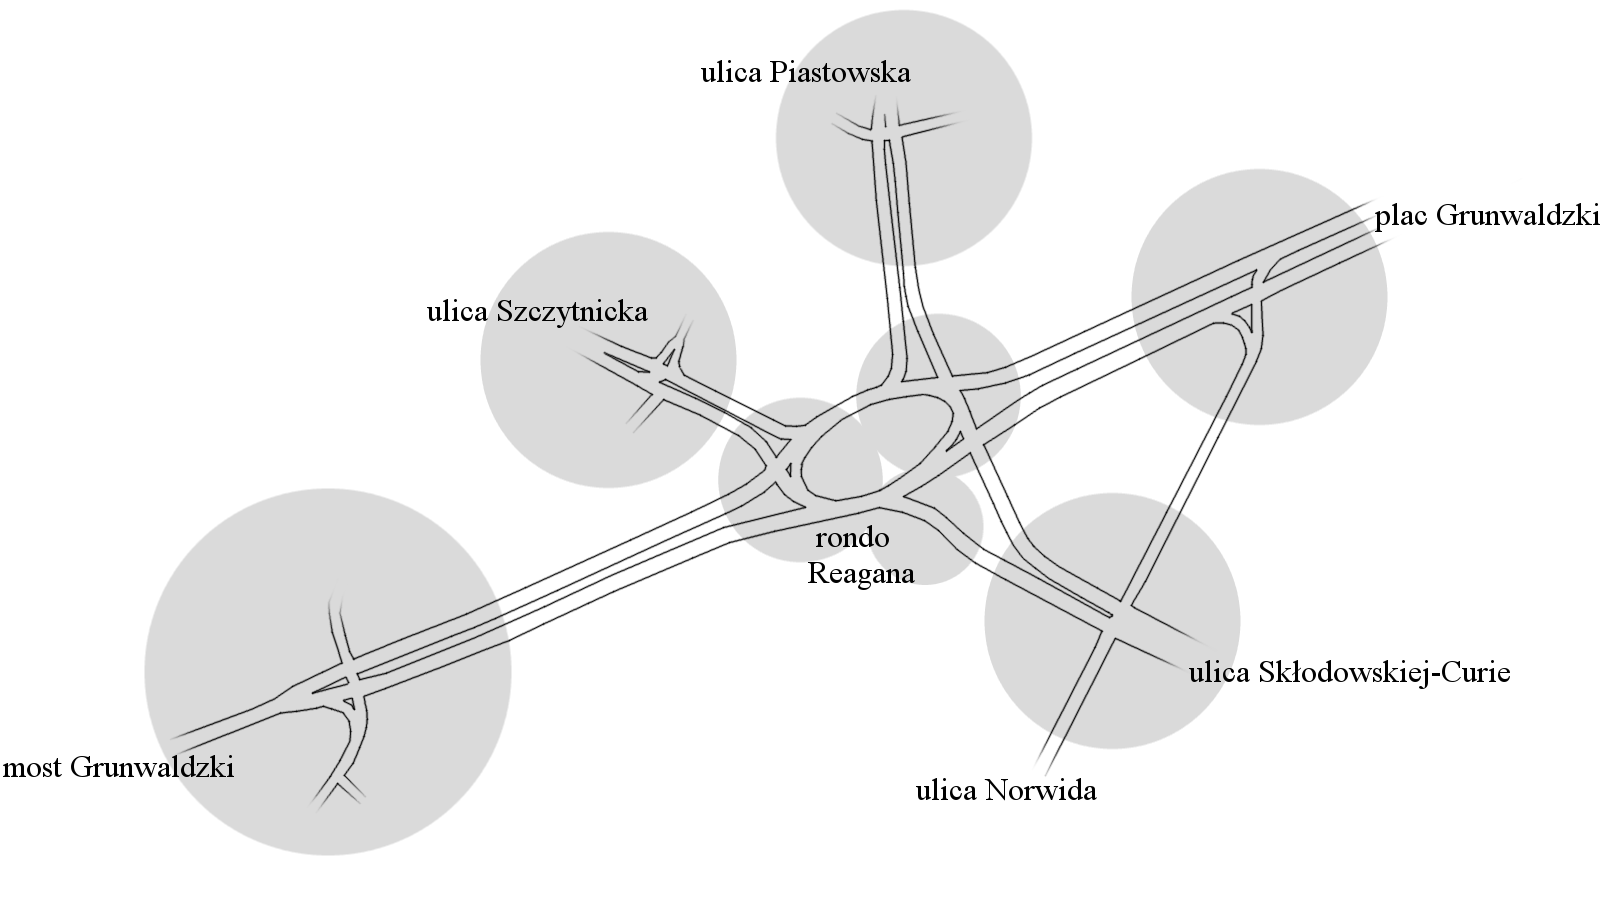
\includegraphics[width=1.0\textwidth]{mapa_czysta.png}
\end{frame}

\begin{frame}[shrink=5]
  \frametitle{\vspace{10px}Wyniki badań\\\small{średnia liczba zatrzymań}}
  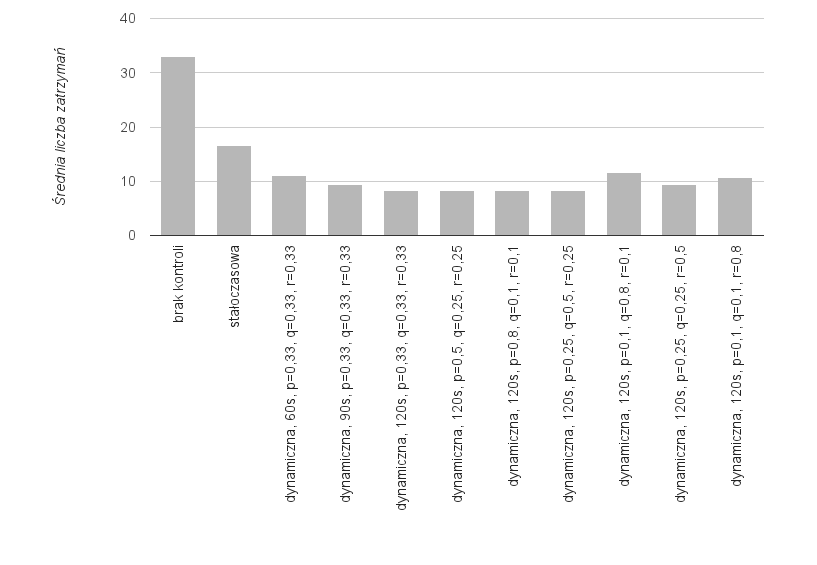
\includegraphics[width=1.0\textwidth]{wyniki_1.png}
\end{frame}

\begin{frame}[shrink=5]
  \frametitle{\vspace{10px}Wyniki badań\\\small{średnia prędkość}}
  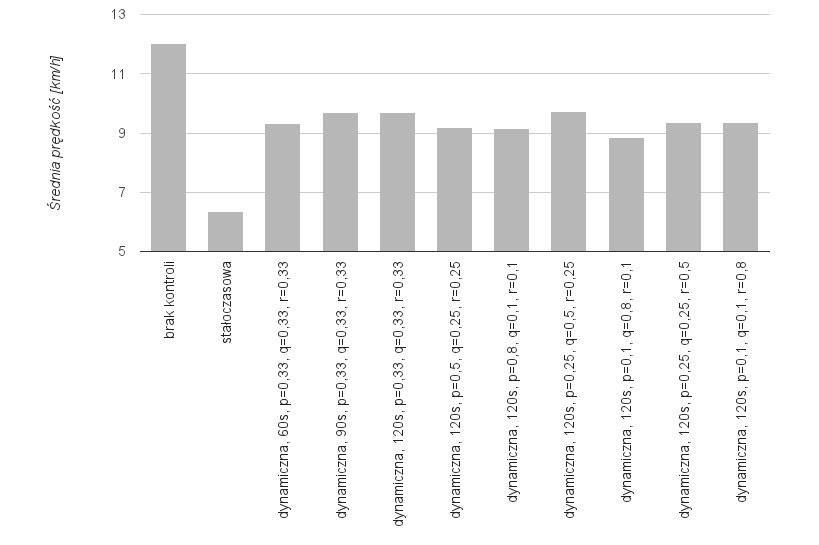
\includegraphics[width=1.0\textwidth]{wyniki_2.png}
\end{frame}

\begin{frame}[shrink=5]
  \frametitle{\vspace{10px}Wyniki badań\\\small{średni czas przejazdu}}
  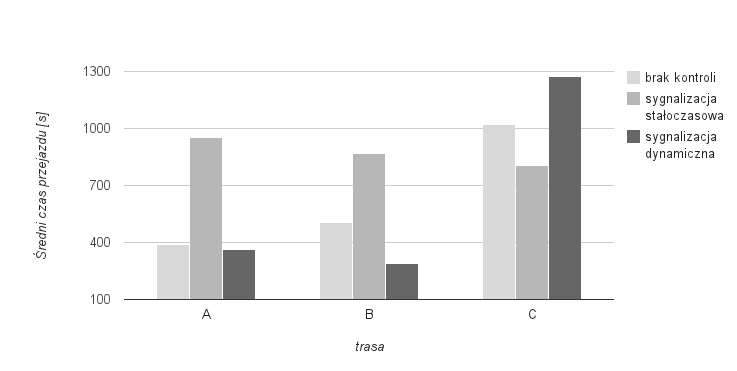
\includegraphics[width=1.0\textwidth]{wyniki_3.png}\\
  \tiny{
  \begin{description}
  \item[trasa A] -- most Grunwaldzki - most Szczytnicki
  \item[trasa B] -- most Szczytnicki - most Grunwaldzki
  \item[trasa C] -- kliniki - most Grunwaldzki
  \end{description}
  }
\end{frame}

\begin{frame}
 \frametitle{\vspace{22px}Wnioski}
  \small{
  \begin{itemize}
    \item zastosowanie algorytmu pozwala na zmniejszenie liczby zatrzymań pojazdów
    \item proponowany algorytm zwiększa średnią prędkość pojazdów w porównaniu z prostym algorytmem sterowania
    \item algorytm pozwala na poprawę czasu przejazdu na dwóch z trzech badanych tras, poprawa wyników na trzeciej trasie wymaga dokładnego dopasowania parametrów
  \end{itemize}
  }
\end{frame}

\begin{frame}
 \frametitle{\vspace{22px}Dziękuję za uwagę}
  \begin{center}Dziękuję za uwagę\end{center}
\end{frame}

\end{document}
